\documentclass{scrartcl}
\usepackage[utf8]{inputenc} 
\usepackage[T1]{fontenc}
\usepackage{lmodern}
\usepackage[ngerman]{babel}
\usepackage{courier}
\usepackage{amsmath}
\usepackage{graphicx}
\usepackage{multicol}
\usepackage{geometry}
\usepackage{authblk}
\usepackage[font=scriptsize, labelfont=bf]{caption}
\usepackage{listings}
\usepackage{hyperref}
\usepackage{color}
\usepackage{amssymb}
\newenvironment{Figure}
  {\par\medskip\noindent\minipage{\linewidth}}
  {\endminipage\par\medskip}
  
\definecolor{dkgreen}{rgb}{0,0.6,0}
\definecolor{gray}{rgb}{0.5,0.5,0.5}
\definecolor{mauve}{rgb}{0.58,0,0.82}

\lstset{frame=tb,
  language=C,
  aboveskip=3mm,
  belowskip=3mm,
  showstringspaces=false,
  columns=flexible,
  basicstyle={\small\ttfamily},
  numbers=none,
  numberstyle=\tiny\color{gray},
  keywordstyle=\color{blue},
  commentstyle=\color{dkgreen},
  stringstyle=\color{mauve},
  breaklines=true,
  breakatwhitespace=true,
  tabsize=3
  }


% for skript letters like H...
\usepackage{mathrsfs}

\geometry{verbose,a4paper,tmargin=25mm,bmargin=25mm,lmargin=15mm,rmargin=20mm}

\title{Protokoll zum Versuch Nichtlineare Dynamik und Chaos}
\author{Nicolas Heimann, Jesse Hinrichsen}
\affil{\textit{Universität Hamburg}}
\date{2015}
\begin{document}
\maketitle
\begin{center}
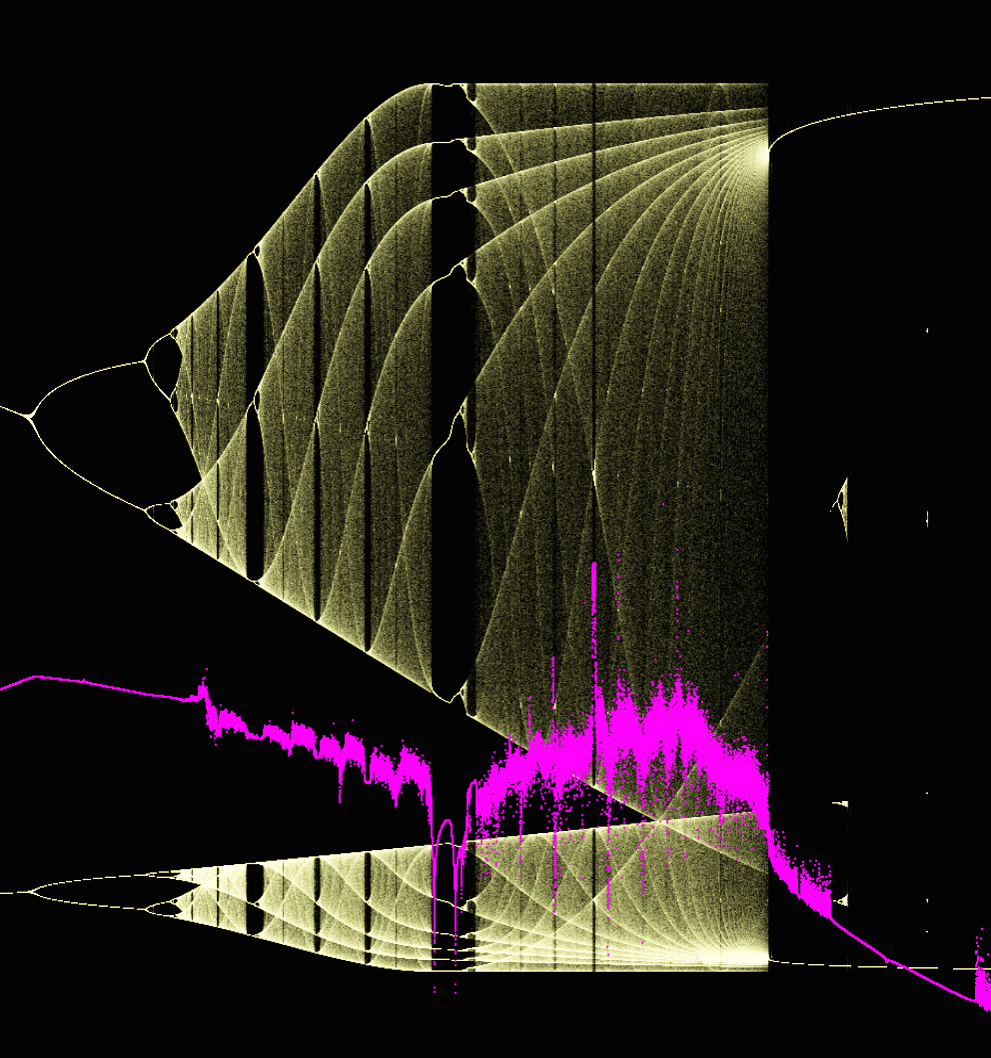
\includegraphics[scale=0.25]{funfunfun} 
\end{center}

\begin{description}
\item ABSTRACT TEXT TODO - vorläufig stand 270815
\end{description}

\section{Einleitung}
Alle Plots und Simulationen in diesem Protokoll haben wir im Rahmen des Versuches selber implementiert. Dafür wählten wir als Programmiersprache Python2.7 und nutzten OpenGL4.1 und OpenCL für Visualisierungen und Berechnungen. Der Quellcode ist online über github einsehbar: \url{https://github.com/keksnicoh/gl_plotting_experimental}. Bei Abbildungen ist ein entsprechender Quellcodeverweis angegeben. 

Im folgenden bezeichnet $f^2(x) = f(f(x))$

\tableofcontents

\section{Logistische Abbildung}
Die logistische Abbildung ist gegeben durch $f(x_n)=x_{n+1}=rx_n(1-x_n)$. Es zeigt sich das diese einfache Funktionsvorschrift 
bereits chaotisches Verhalten an den Tag legt welches wir im folgenden Abschnitt genauer untersucht haben. Zunächst haben 
wir ein Bifurkations Diagramm der logistischen Abbildung erzeugt indem wir den Parameter r gegen Iterationspunkte aufgetragen haben. Dabei fixierten wir jeweils ein r und erzeugten eine Folge $x_0 ... x_{1000}$ von welcher wir $x_{500} ... x_{1000}$ auf die y-Achse aufgetragen haben (Abbildung \ref{fig:bifurkation-sin-nice}).
Das Bifurkationsdiagramm lässt sich in mehrere Bereiche unterteilen. Bis $r=3$ laufen die $x_{500}...x_{1000}$ auf den gleichen Fixpunkt zu. An $r=3$ gabelt sich das Diagramm in zwei Äste auf (Periodenverdoppelung). An $r=3.449$ gibt es eine weitere Perdionenverdopplung und es ist eine Selbstähnlichkeit mit dem Bereich um $r=3$ zu erkennen (Fraktale Strukturen). Ab $r=3.569$ entsteht ein chaotischer Bereich in welchem sich aber noch Strutkuren feststellen lassen (Bögen, Punkte auf geraden, freie Bereiche).
\begin{figure}
	\centering
	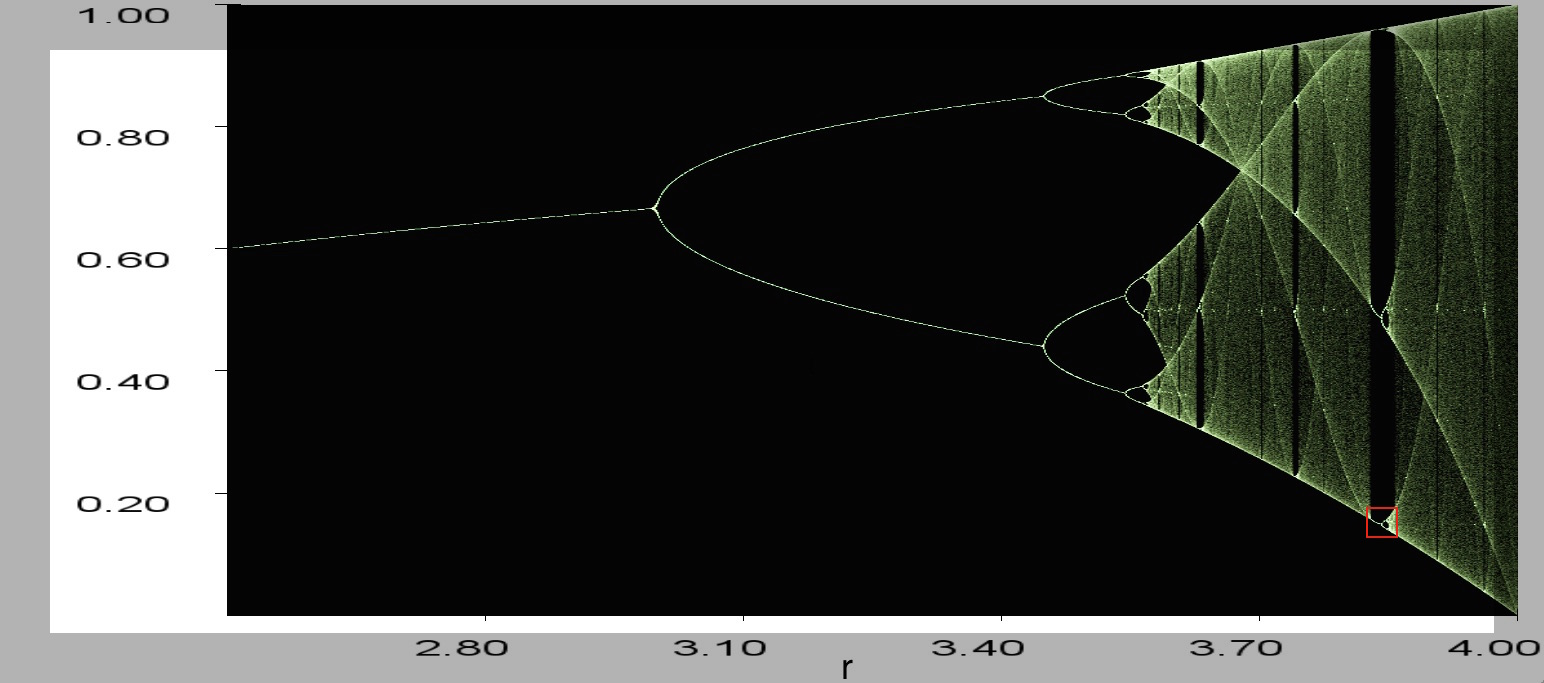
\includegraphics[scale=0.30]{bifurkation}
	\caption{Bifurkationsdiagramm der logistischen Abbildung im Bereich $r\in[2.6,4]$. sourcecode: prak/birukation-logistisch-no-opt.py}
	\label{fig:bifurkation-sin-nice}
\end{figure}
\subsection{Fixpunkte / Stabilitätsbedigung}
Bildet die Funktion einen Punkt idempotent ab, so handelt es sich um einen Fixpunkt, es gilt: $f^n(x^*)=x^* \forall n \iff x^* ist Fixpunkt$. 
Stabilitätsbedingung
$$|f'(x^*)|<1 \iff Fixpunkt-stabil$$
$$|f'(x^*)|>1 \iff Fixpunkt-instabil$$ Mit
\begin{math}
f(x^*)=rx^*(1-x^*)=x^*
\iff x^*=1-1/r \vee x'=0
\end{math}
ließ sich so analytisch bestimmen, dass die Fixpunkte für $r \in [0,1) \cup (3,4]$ instabil für $r \in (1,3)$ stabil sind.
Obwohl für den Parameter $0 \textless r \textless 1$ der Fixpunkt instabil ist konvergieren $f^n(x)$ gegen 0 $\forall x \neq x^*$, denn $f^n(x)$ ist ein Polynom vom grad $2n$. 


Abbildung \ref{fig:log-iteration-behavior} zeigt wie sich die Iteration jeweils für einen stabilen und einen Instabilen Fixpunkt verhält. So lässt sich auf die Aufspaltung im Bifurkationsdiagramm (Abbildung \ref{fig:bifurkation-sin-nice}) für $r>3$ verstehen.  
Für den Zweierzyklus $f^2(x)$ ließen sich folgende Fixpunkte bestimmen welche in Abbildung \ref{fig:log-intermittenz-cycles} zusammen mit dem Einerzyklus Fixpunkten dargestellt sind ermitteln. 
Die logistische Funktion zeigte bei einigen Parametern r Intermittenz (Abbildung \ref{fig:log-intermittenz-cycles}). Intermittenz ein Grund für die Verdichtungen welche im choatischen Bereich des Bifurkationsdiagrammes zu sehen sind.

$$x_{n+1}=f_r(x_n)=rx_n(1-x_n)$$
$$\Rightarrow x_{n+2}=r^2x_n(1-x_n)(1-rx_n(1-x_n))$$
\newline
Fixpunktgleichung (Zweierzyklus):
$$x=r^2x(1-x)(1-rx(1-x))$$
$$\Rightarrow x_{3,4}=\pm\frac{\sqrt{r^2-2 r-3}+r+1}{2 r}$$
Damit $x_{3,4}$ reel bleibt muss $r^2-2 r-3 \geq 0$
$$\Rightarrow r \leq -1 \land r \geq 3$$
Für diesen Bereich gibt es folglich 2 weitere Fixpunkte $x_{3,4} 
\Leftrightarrow$ Perdiodenverdopplung. 
Im Fall der logistischen Abbildung gilt
$$\frac{d}{dx}f(x)=r-2rx=r(1-2x)$$
$$\frac{d}{dx}f^2(x)=-r^2(2x-1)(2r(x-1)x+1)$$
AB HIER TODO: Grafisch lässt sich ablesen, dass der Fixpunkt $x_3=\frac{\sqrt{r^2-2 r-3}+r+1}{2 r}$ (grüner Graph) für folgende Bereiche stabil ist:
$$-1.45<r<-0.82 \Rightarrow -1.45 < r \leq -1$$
$$2.82<r<3.45 \Rightarrow 3 \geq r > 3.45$$
Der Fixpunkt $x_4=\frac{-\sqrt{r^2-2 r-3}+r+1}{2 r}$ (grauer Graph) ist im gesamten Bereich $-1.45<r<3.45$ stabil aber da der Fixpunkt ebenfalls nur für $r \leq -1 \land r \geq 3$ existiert gilt der selbe Bereich wie für $x_3$. Die Fixpunkt sind dort stabil, wo sich der graue und der grüne Graph in der Abbildung überlagern.



\begin{figure}
\centering
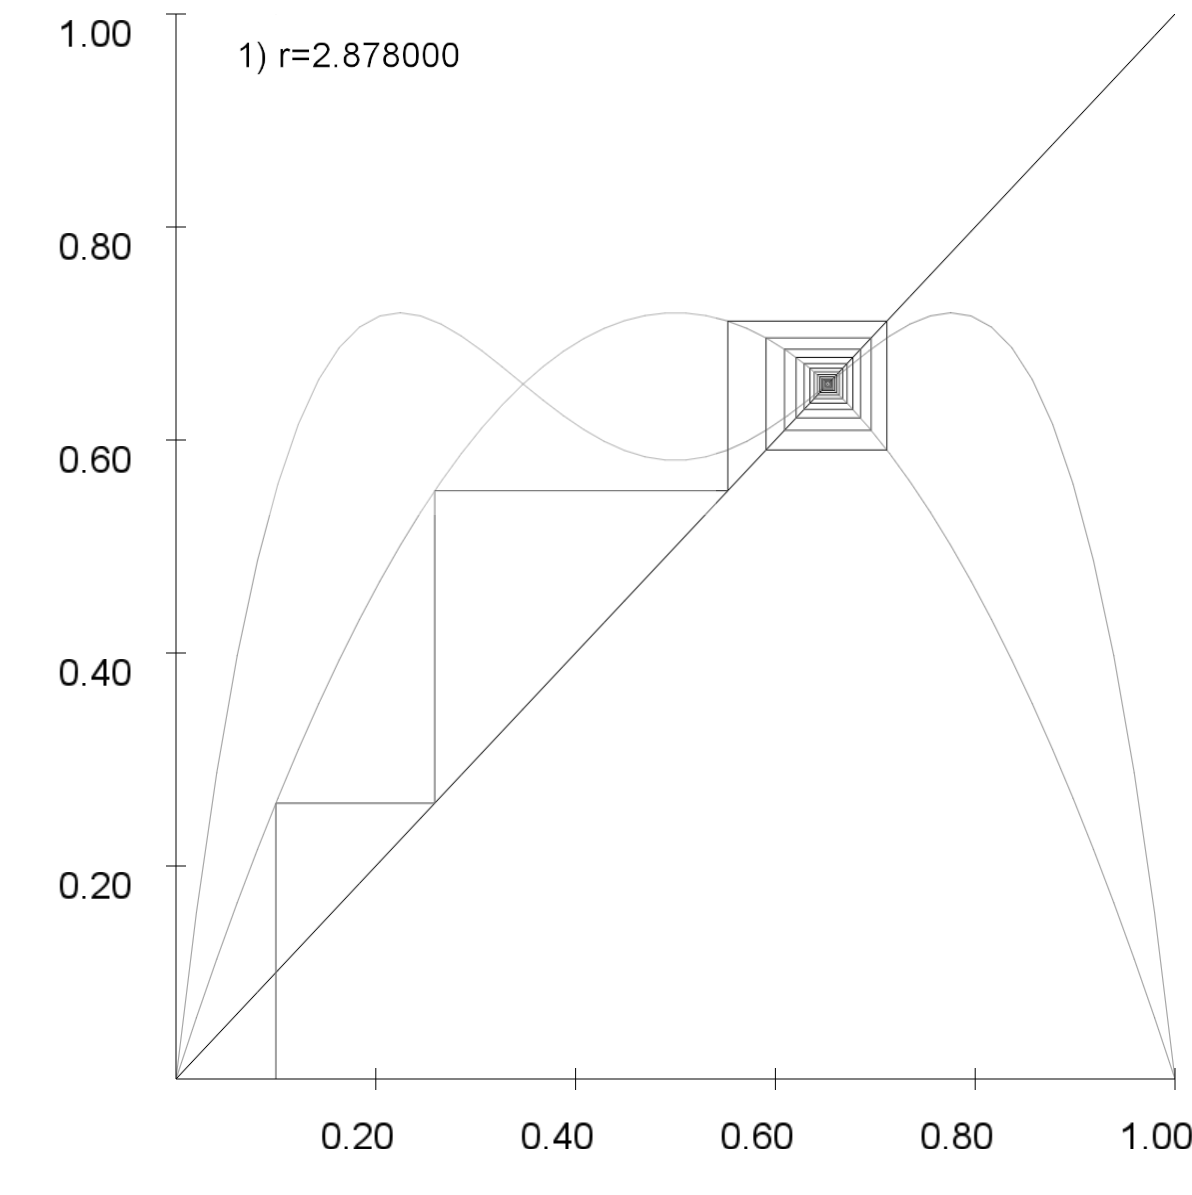
\includegraphics[scale=0.2]{fixpunkt-2878}
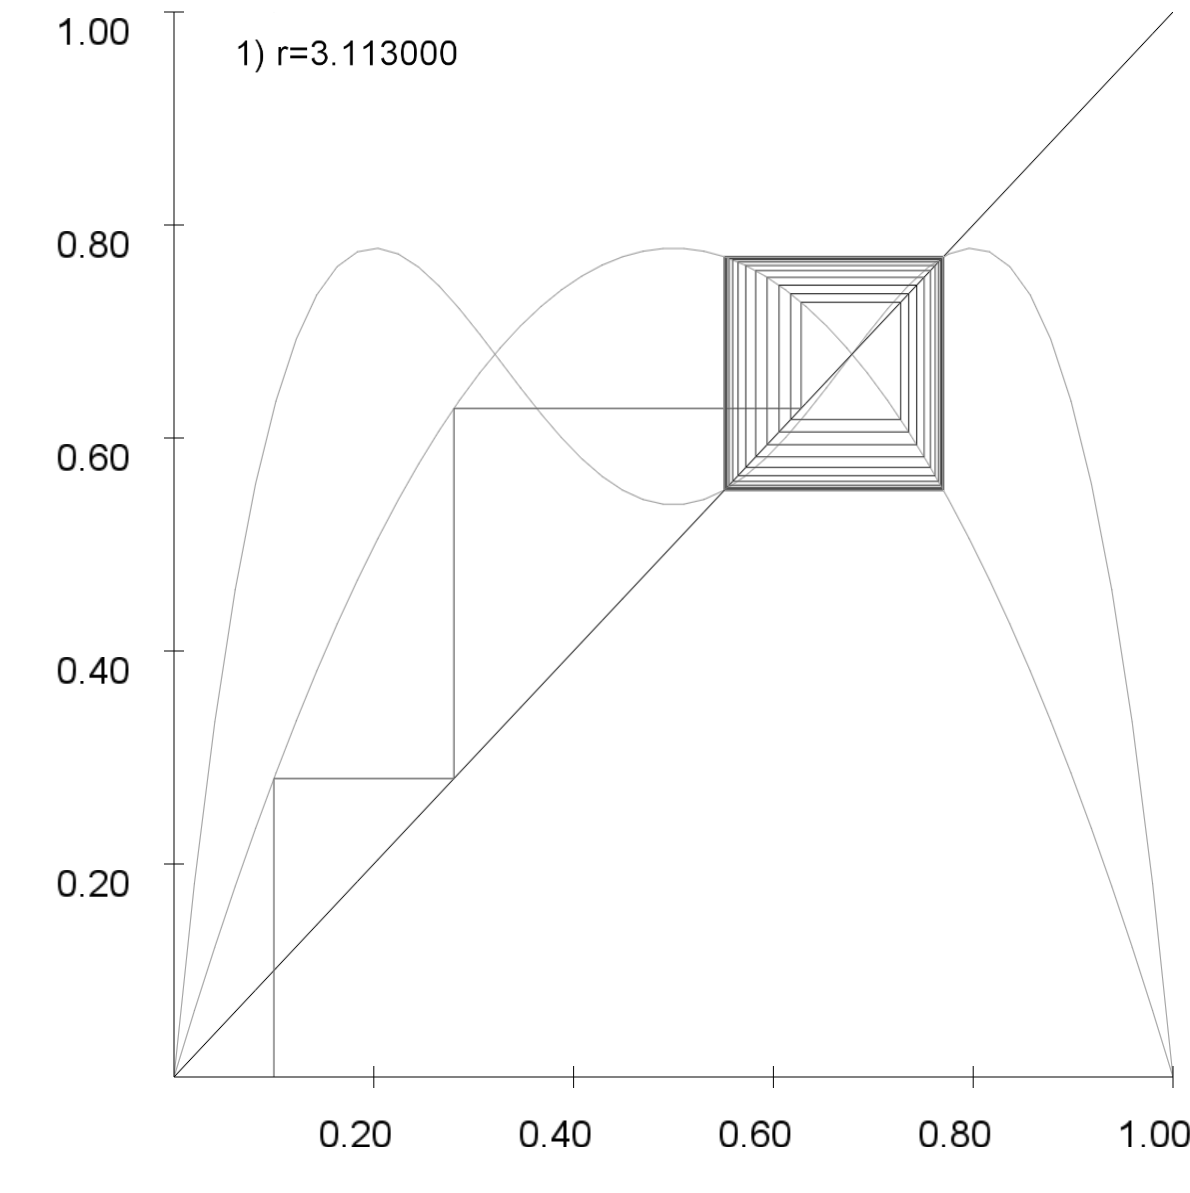
\includegraphics[scale=0.2]{fixpunkt-311}
\caption{Verlauf der Iterationen bei festen Parameter r. Linkes Bild zeigt einen stabilen Fixpunkt bei r=2.878, rechtes Bild zeigt instabilen Fixpunkt bei r=3.113. Der Verlauf der logistischen Funktion $f(x)$, $f^2(x)$ sowie die Einheitsgerade $y=x$ sind aufgetragen . Als Linie Verbunden geplottet ist die Folge ($x_n, 0.0), (x_n, x_{n+1}), (x_{n+1}, x_{n+1}), (x_{n+1}, x_{n+2}), (x_{n+2}, x_{n+2}), (x_{n+2}, x_{n+3}), ...$ Sourcecode: prak/logisitsch-no-opt-behavior.py}. 
\label{fig:log-iteration-behavior}
\end{figure}

\begin{figure}
\centering
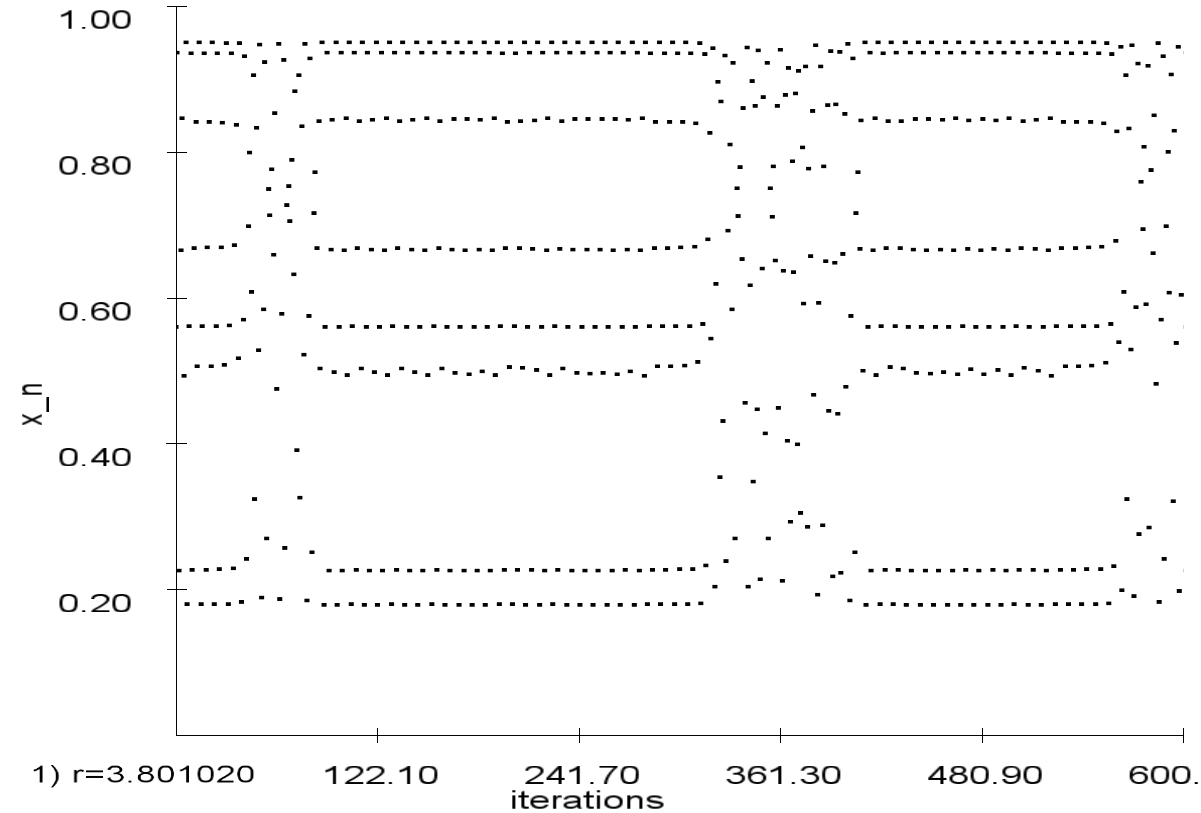
\includegraphics[scale=0.22]{intermittenz}
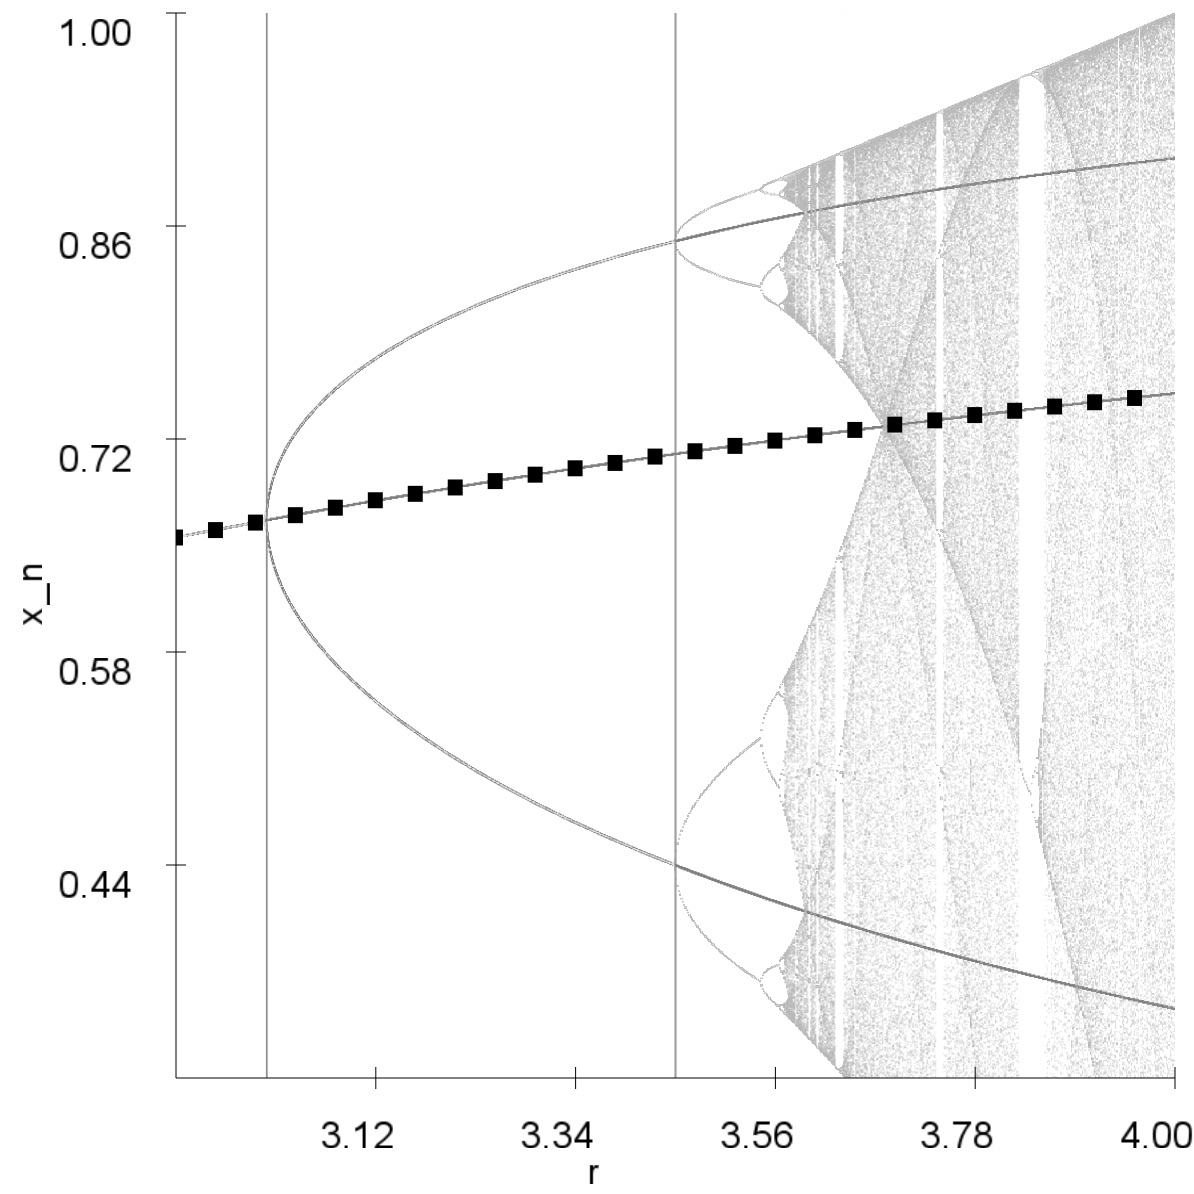
\includegraphics[scale=0.15]{analy-periodenv}
\caption{Logistische Funktion. Links: Intermittenz bei $r=3.80102$. Rechts: Die stabile Lösung des Einerzyklus $x^*$ und die beiden Lösungen des Zweierzyklus $x_{3,4}$. Im Hintergrund das Bifurkationsdiagramm. Die vertikalen Linien sind an $r=3.0$ und $r=444$ und markieren die Stellen wo $|f'(x)|=1$, $|\frac{d}{dx}f^2(x)|=1$ sind. Sourcecode: prak/intermittenz.py, prak/logis-zyklen.py}. 
\label{fig:log-intermittenz-cycles}
\end{figure}


\subsection{Lyapunov Exponent}
Der Lyapunov Exponent beschreibt mit welcher Geschwindigkeit sich zwei naheliegende Punkte voneinander entfernen. 
Es gibt drei Wege den Lyapunov Exponenten zu implementieren:

(1) Definition
$\lambda(x_0) = \lim_{N \rightarrow \infty}\lim_{\epsilon \rightarrow 0} \frac{1}{N}\log{\mid \frac{f^N(x_0+\epsilon)- f^N(x_0)}{\epsilon} \mid} $


(2) Analytisch
$\lambda(x_0) = \lim_{N \rightarrow \infty} \frac{1}{N} \sum_{i=0}^{N-1}  \log{f'(x)} $


(3) Renormiert:
Nach jedem Iterationsschritt wird der Abstand $\epsilon$ neu gesetzt. \newline

In Abbildung \ref{fig:lyapunov} haben wir die drei Möglichkeiten auf die logisitsche Funktion angewendet.
Es zeigte sich, dass die erste Möglichkeit sehr schlechte Ergebnisse im Vergleich zu den beiden letzten Methoden ergibt.
Dies liegt daran, dass die selbt bei kleinen $\epsilon$ die Funktionswerte sehr schnell divergieren und somit die Definition des Differenzenquotienten keinen Sinn ergibt.
Die Renomierung hält diesen Abstand in jedem Iterationsschritt klein, weshalb sich der Lyapunov Exponent trotzdem ausrechnen lässt.
Der Lyapunov Exponent hat seine Nullstellen dort wo die Abbildung ihre superattraktiven Stellen hat. Umgekehrt divergiert $\lambda(x_0)$ an den superattraktiven Stellen.
Man erhält also Information über das Verhalten der Abbildung für bestimmte $x_0$.
Tratsächlich kann man den Lyapunov-Exponenten über den mittleren Informationsverlust ausdrücken $\lambda(x_0)=-log(2)*\delta I$ (QUELLE skript todo).
Im folgenden ist der OpenCL Quellcode der renomierten Formel des Lyapunov Exponenten:
\begin{lstlisting}
float g(float r, float x) {
    return r * x * (1-x);
}
vec4 f(vec4 x) {
    float x0 = 0.4;
    float eps = 0.0001;
    float n = 10000;
    float summe = x0;
    for (int i=1; i < n; i++) {
        x0 = g(x.x, x0);
        summe += log(abs(g(x.x, x0+eps)-g(x.x, x0))/eps);
    }
    return vec4(x.x, summe/n, 0, 0.5);
}
\end{lstlisting}
\begin{figure}
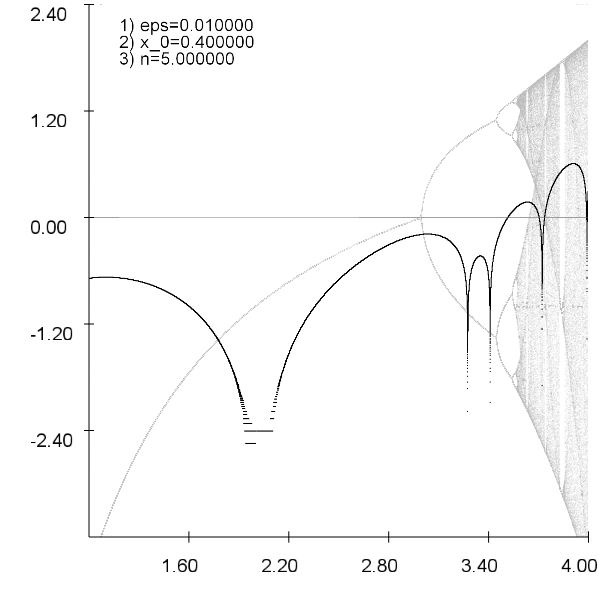
\includegraphics[scale=0.28]{iteration/lyapunov-1}
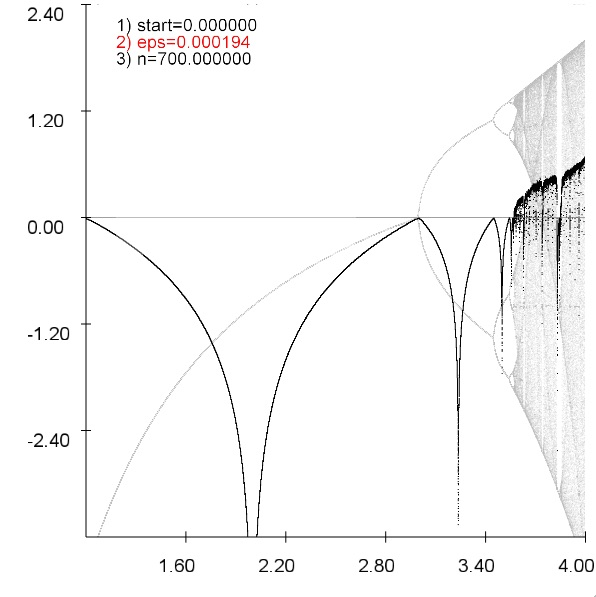
\includegraphics[scale=0.28]{iteration/lyapunov-2}
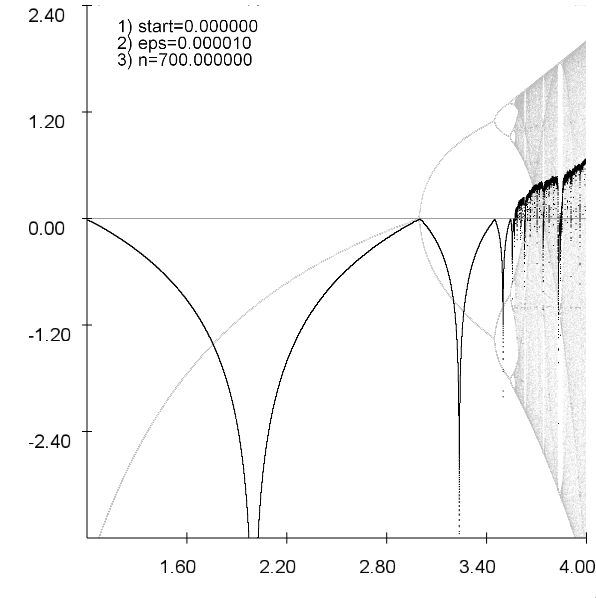
\includegraphics[scale=0.28]{iteration/lyapunov-3}
\caption{Drei verschiedene Implementation des Lyapunov Exponent. Links: Definition, Mitte: Analytisch, Rechts: Renormiert. Die linke Implementation weißt deutliche Abweichungen im Vergleich zu den anderen beiden Implementation auf und ist somit unbrauchbar. Sourcecode: prak/lyapunov.py}. 
\label{fig:lyapunov}
\end{figure}
 
\subsubsection{Betrachtung im chaotischen Bereich.}
In Abbildung \ref{fig:lyapunov} ist zu sehen wie der Lyapunov Exponent ab $r=...$ zu rauschen beginnt. 
Der Verdacht liegt nahe, dass nicht genuegend Iterationsschritte zur Berechnung ausgeführt wurden also erhöhten wir die Anzahl an Iterationen für die Berechung von $\lambda(x)$. Es zeigte sich allerdings kaum eine Veränderung. Die Frage nach der Konvergenz von $\lambda(x)$ im chaotischen Bereich galt es zu untersuchen: Abbildung \ref{fig:lyapunov-chaos} zeigt das Langzeitverhalten von $\lambda(x)$ über $19*10^6$ Iterationen. $\lambda(x)$ erinnert die ersten $10^7$ Iterationen eher an einen Börsenkurs und nicht an ein Objekt welches gegen einen Grenzwert konvergiert. Erst nach ca. $10^7$ Iterationen deutet sich Konvergenzverhaltens an. Dieses ist aber nicht sehr präzise: Falls 
$$
\lim_{N \rightarrow \infty} \lambda_N(x) = L
$$
so kann man nach $2*10^7$ Iterationen höchstens feststellen, dass der Graph in einem Epsilon Schlauch von $\epsilon=0.002$ passt. Dies ist nicht sehr befriedigend angesicht der massiven Iterationslänge.  

TODO: Optimierungen?

TODO: was passiert bei r>4.0

\begin{figure}
\centering
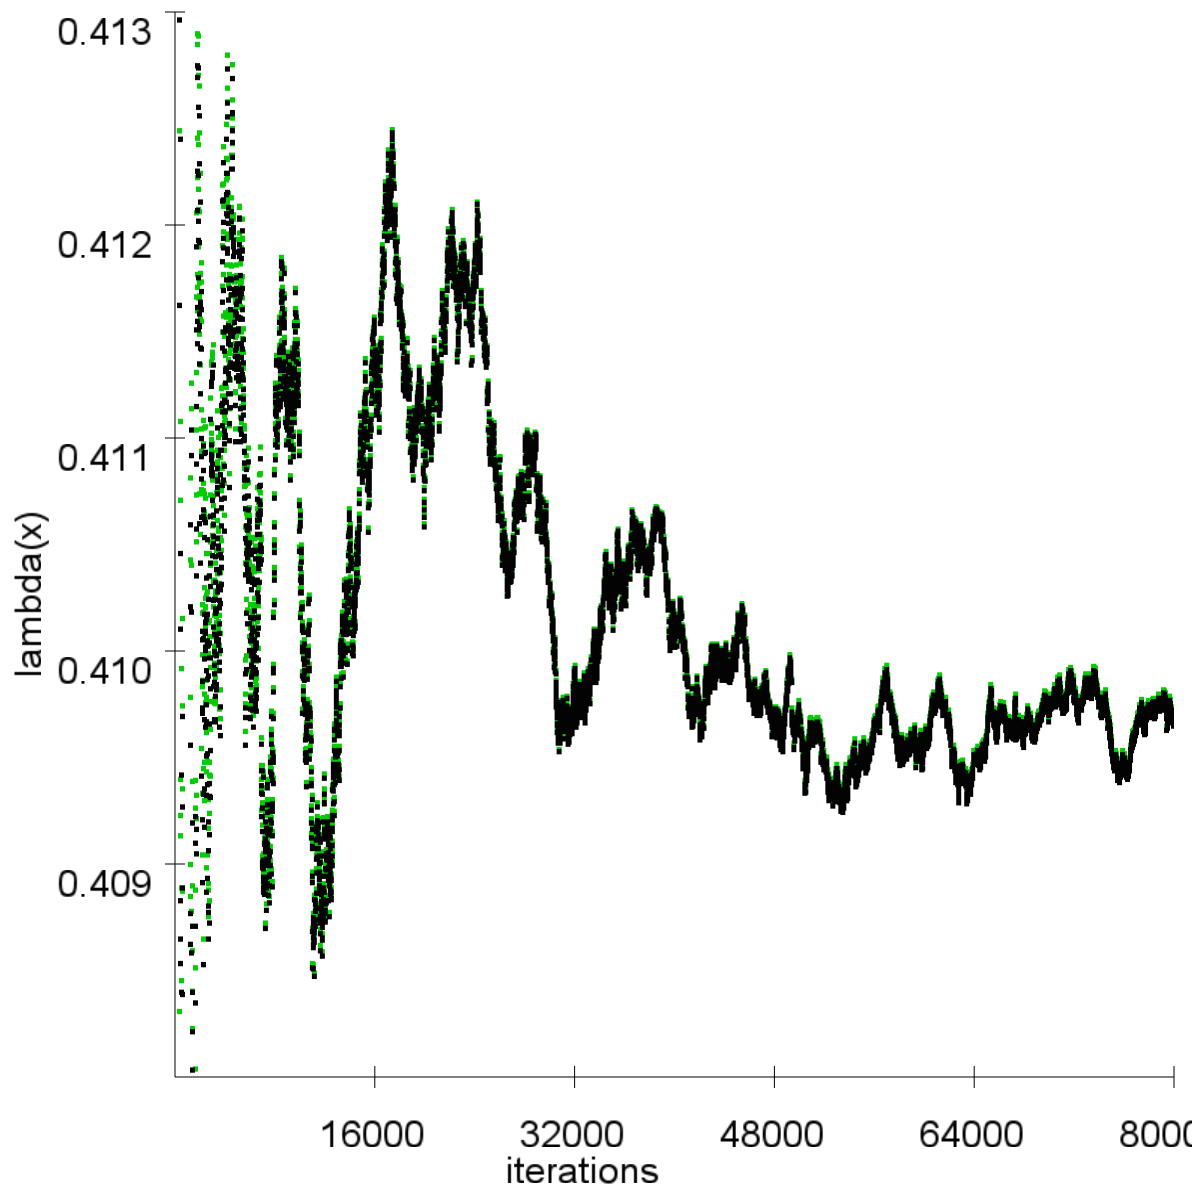
\includegraphics[scale=0.18]{lya378-zoom}
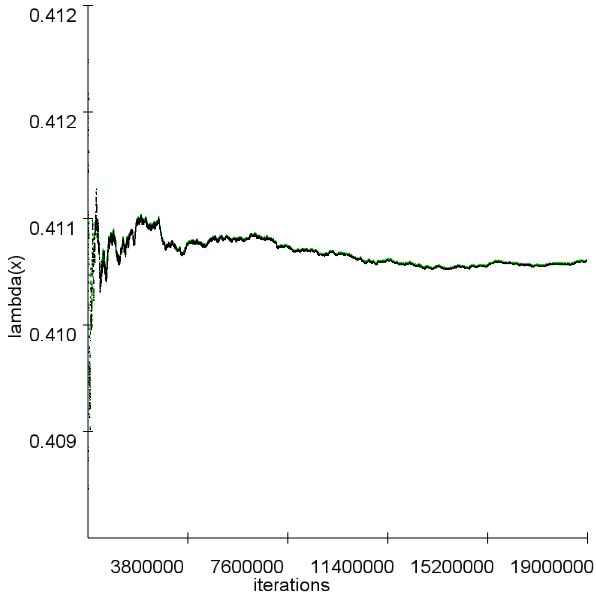
\includegraphics[scale=0.36]{lya378}
\caption{Analytische(schwarz) und renormierter(grün) Lyapunov Exponent im chaotischen Bereich bei $r=3.78$. Links: Zoom im Bereich 0 bis $80*10^3$ Iterationen. Rechts:  0 bis $19*10^6$ Iterationen.}
\label{fig:lyapunov-chaos}
\end{figure}


\subsubsection{Vergleich der analytischen und renomierten Implementation}
Wir haben nun die analytische und die renormierte Implementation des Lyaponovexponenten weiter untersucht. Dabei stellten wir fest, dass bei Stellen mit Periodenverdoppelung die renormierte Formel etwas schneller gegen die 0 konvergiert als die analytische Formel. An einer weiteren Stelle ($r=3.05$) ist zu erkennen wie beide Implementationen einmal von oben (renormiert) und ein mal von unten (analytisch) gegen einen scheinbar gemeinsamen Wert streben (Abbildung \ref{fig:lyapunov-compare}). Die Vermutung liegt nahe, dass man mit dem Mittelwert aus beiden Implementationen an solchen stellen wesentlich schneller den Grenzwert bestimmen kann. Es zeigt sich aber, dass dieses Verhalten nicht regelmäßig auftritt weshalb wir es nicht weiter untersucht haben. Nach weiteren Stichproben scheint die analytische Implementation bis zum 500ten Iterationsschritt etwas schneller als die renormierte Implementation zu konvergieren. Beide Versionen zeigten aber in allen Stichproben $r<3$, dass sie stets gegen den gleichen Grenzwert strebten.
\begin{figure}
\centering
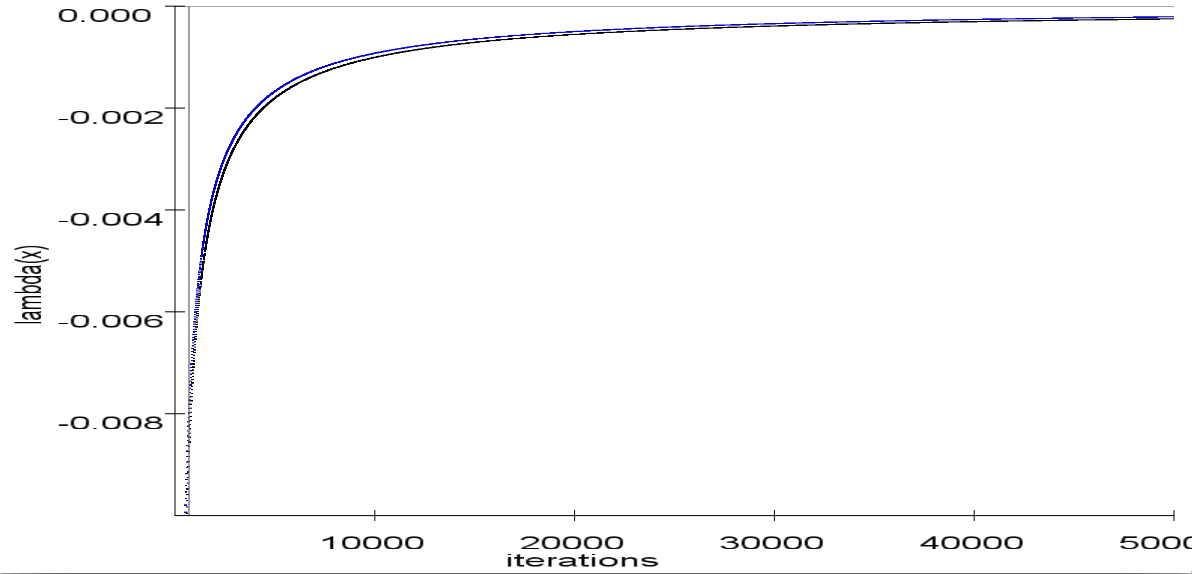
\includegraphics[width=220px, height=220px]{lyapunov-analysis-300}
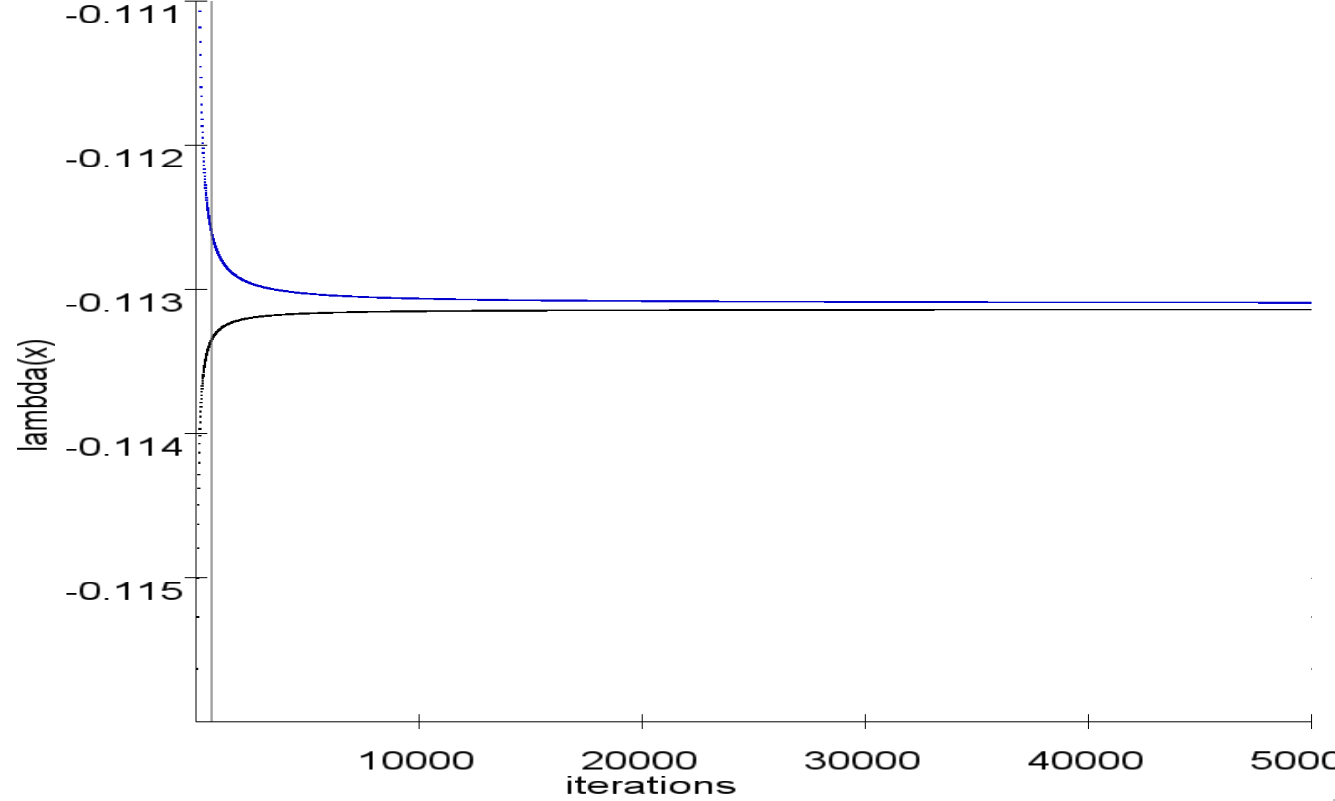
\includegraphics[width=220px, height=220px]{lyapunov-analysis-305}
\caption{Vergleich des analytischen(Schwarz) und renormierten(Blau) Iterationsverhalten des Lyapunov Exponenten. Vertikale Linie bei N=700. Oberes Bild zeigt Iterationsverhalten bei $r=3.0$. Unteres Bild zeigt Iterationsverhalten bei $r=3.05$ }. 
\label{fig:lyapunov-compare}
\end{figure}


\begin{figure}
\centering
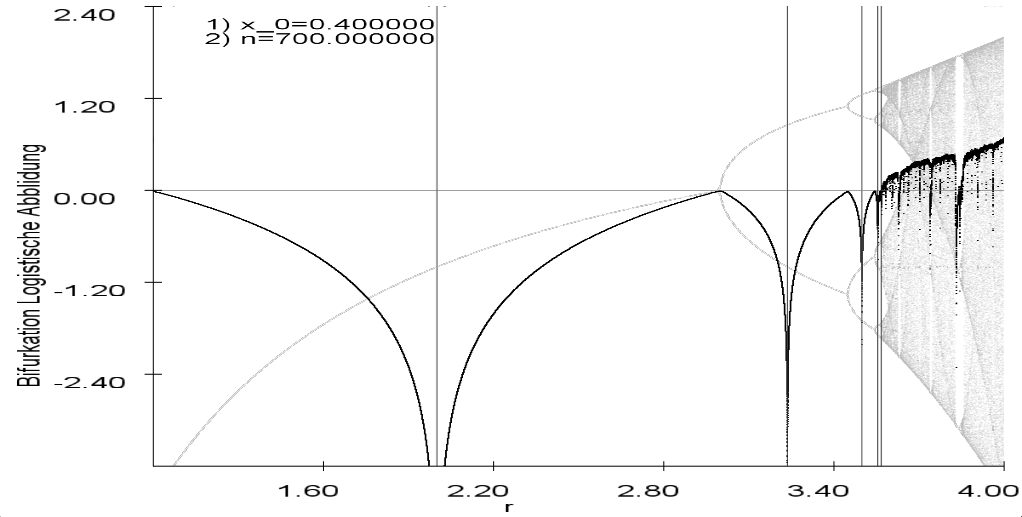
\includegraphics[scale=0.45]{iteration/bifurk-log-lyapunov-periode}
\caption{Analyse des Bifurkationsdiagrammes der logistischen Funktion. Eingezeichnet sind die y=0 Achse, sowie die ersten 5 Superattraktiven Stellen für r. Das Bifurkationsdiagramm wurde so translatiert und skaliert, dass es hinter dem Lyapunov Exponenten erscheint.}. 
\end{figure}





\subsection{Feigenbaumkonstante}
Die Feigenbaumkonstante ist eine universelle Größe. Sie tritt in chaotischen nicht linearen System auf und lässt sich wie folgt bestimmen:
$$\delta_i = \frac{b_i-b_{i+1}}{b_{i+1}-b_{i+2}}$$ oder $$\delta_i = \frac{s_i-s_{i+1}}{s_{i+1}-s_{i+2}}$$
$$\delta = \lim\limits_{i \rightarrow \infty}{\delta_i} = 4.669201609102991 (2.3.1) $$ (TODO QUELLE https://oeis.org/A006890)
wobei $s_i, b_i$ die Folgen der superattraktiven und periodenverdoppelden Stellen sind.
Also lässt sich die Feigenbaumkonstante mit dem Lyapunov Exponenten bestimmen. 
Als erstes haben wir versucht die Nullstellen des Lyapunov Exponenten zu bestimmen. Wir wendeten dabei das folgende Kriterium für eine Nullstelle an:
$$\lambda(x-\epsilon) < \lambda(x) \wedge \lambda(x+\epsilon) < \lambda(x) \wedge |\lambda(x)|<\epsilon$$
Es zeigte sich aber, dass bei genauen Betrachten des numerisch bestimmten Lyapunov Exponenten sehr große Schwankungen vorhanden waren, weshalb dieses Kriterium nicht mit unseren Verfügbaren Rechenleistungen praktikabel war (Abbildung N).
Aufgrund dieser Probleme
haben wir uns dazu entschieden die superattraktiven Stellen anstelle der Bifurkationspunkte numeritsch zu bestimmen. Unser Algorithmus startet im Suchmodus bei gegeben Startwert $x_{start}$ und geht in kleinen Schritten $\Delta x$ die x-Achse ab. In jedem Schritt wird $l_1=\lambda(x_0)$ $l_2=\lambda(x_0 + \Delta x)$ berechnet. 
Ist
$$l_2-l_1 \leq 0 (1) $$
wandert der Iterationsschritt zum superattraktiven Fall. 
Dies wird so lange fortgesetzt bis die Bedingung $(1)$ nicht mehr hält. 
Es wird nun um $\Delta x$ zurückgegangen und anschließend die Schrittweite $\Delta x \mapsto \frac{\Delta x}{10} $ verkleinert. Nun wird erneut so lange iteriert, bis $(1)$ nicht mehr hält. 
Der Vorgang wiederholt sich 8 mal. Anschließend wird $(2*x_0 + \Delta x )/2$ als Ergebniss gespeichert. 
Als nächstes befindet sich der Algorithmus im Anfangspunkt-Modus. Es wird so lange die x-Achse abgetestet bis die Bedingung 
$$\lambda(x_0) < \lambda(x_0 + \Delta x) < \lambda(x_0 + 2*\Delta x)$$
nicht mehr erfüllt ist und somit ein neues $x_{start}$ gefunden wurde. Der Suchmodus wird aktiviert.  (Quellcode: prak/feigenbaum.py)
Im folgenden ist die Terminal Ausgabe des Algorithmusses beigelegt:
\begin{lstlisting}
searching from 1.9
looking for next start_r from 2.00000000002
searching from 2.99950000003
looking for next start_r from 3.23606797751
searching from 3.44927797752
looking for next start_r from 3.49856169934
searching from 3.54400769935
looking for next start_r from 3.55464086278
searching from 3.56439786279
looking for next start_r from 3.56666737986
found values [2.0000000000249916, 3.236067977509959, 3.498561699344952, 3.554640862779951, 3.5666673798649517]
delta_0=4.70894301336
delta_1=4.68077099865
delta_2=4.66295961155
\end{lstlisting}
Somit konnten wir numerisch für $i=2$ eine Feigenbaumkonstante von $\delta_2=4.66295961155$ berechnen. Dieser Wert weicht um 0.133671789\% vom tatsächlichen Wert (2.3.1) ab. Die Grenzen des Algorithmus sind bereits nach 5 gefunden superattraktiven Stellen erreicht. Ab $r>3.57$ fängt die numerische Implementation des Lyapunov Expontenten an zu "rauschen" (Abbildung N). Der Algorithmus kann daher nicht mehr präzise seinen Suchmodus ausführen. Ebenfalls liegen die nächsten Superattraktiven Fällen noch dichter bei Sammen als es für $s_4$, $s_5$ der Fall war, was ebenfalls vom Algorithmus nicht mehr detektiert wird. 

\section{Sinus Abbildung}
Die Sinusabbildung ist gegeben durch 
$$f(x_n)=x_{n+1}=r*sin(x)$$
Wir haben die bereits implementierten Programme nun auf die Sinus Funktion angewendet. Abbildung \ref{fig:bifurc-sin} zeigt das Bifurkationsdiagramm der Sinusabbildung. Es fällt sofort auf, dass sich die Bildpunkte innerhalb einer Einhüllenden befinden. Betrachtet man die Funktion wird wegen des Bildbereiches des Sinus ($[-1,1]$) sofort klar, dass $\sup_{n \in \mathbb{N}} |f^n(r)| \leq r $ gilt. Bei den Bifurkationsdiagrammen der logistischen Abbildung hatten wir ein festen Startwert $x_0$ gewählt. Für die Sinusabbildung wählten wir als Startwerte die Folge $x_{0,n} = (-1)^n * x_0$ da sonst im Bereich $r \in [0,\pi]$ das Bild des Graphen stets positiv wäre. Auch dieses Phänomen lässt sich mit einfachen Überlegungen erklären: 
$$sin([0,\pi]) = [0,1] \Rightarrow f([0,\pi]) = [0,\pi] \Rightarrow f^2([0,\pi]) = [0,\pi] \forall r \in [0,\pi]$$
 
Das Anwenden unseres Algorithmuses zur bestimmung der Feigenbaumkonstante lieferte im Vergleich zur logistischen Abbildung keine guten Ergebnisse. Die ersten superattraktiven Stellen $s_i$ ließen sich ohne weiteres bestimmen. Die Abstände $\Delta s$ werden schon nach den ersten 4 Folgegliedern sehr klein und der Lyapunov Exponent beginnt zu "rauschen". 
Wir entwickelten einen weiteren Algorithmus, welcher nur maginal bessere Ergebnisse nach $s_4$ lieferte. Die Idee des Algorithmusses war es, zunächst den Lyapunov Exponenten Grob für $r\in [0,3.2]$ zu berechnen. 
Die so entstandene Folge $l_i=(x_i, l(x_i))$ wird nun iteriert. Sobald $l_{i,1} < M < 0$ gilt wird $A=l_{i,0}$ gesetzt. Es wird weiter iteriert bis $l_{i,1} > 0$ und schließlich wird das Intervall $[A, l_{i,1}]$ gespeichert. Dies wird bis zum Ende der Folge $l_i$ ausgeführt. 
Nun wir der Algorithmus für eine tiefere Schranke auf alle ermittelten Intervalle erneut angewendet. 
Wir fanden so mehrere Hinweise auf die nächsten superattraktiven Stellen. 
Schließlich wurde $M \leq 4.0$ und plötzlich fielen keine Punkte außer $s_1, s_2, s_3, s_4$ in das Raster. Beim betrachten des Lyapunovexponenten fiel auf, dass trotz einer Iterationstiefe von 10000 Iterationen stets galt $\lambda(x)>-4.0$. 
Wir haben dafür nur zwei plausible Erklärungen: 
(1.) $s_5-s_4$ ist sehr klein und wir erwarten, dass $s_6-s_5$ noch kleiner ist (untere Abbildung \ref{fig:bifurc-sin}). Eventuell reicht unsere numerische Genauigkeit nicht aus. 
(2.) Die sinus Funktion ist ungenau implementiert und verschmiert so den Grenzwert. 
Die folgenden superattraktiven Stellen haben wir besimmt: $s_1=0.0$, $s_2=1.570728749999546$ $s_3=2.4432446071429674$, $s_4=2.6580499999998904$, $s_5=2.70599999999986$, $s_6=2.71600010303040$ und daraus die ersten 4 Glieder in der Feigenbaum Folge bestimmen:
$$\delta_1=1.8002294596$$
$$\delta_2=4.06188990667$$
$$\delta_3=4.47977878743$$
$$\delta_4=4.79495059736$$

Anders als die logistische Abbildung bricht das Bifurkationsdiagramm der Sinusfunktion nicht ab. Auch dies lässt sich auf den Kompakten Bildbereich des Sinus zurückführen. Der Lyapunov Exponent weißt ab $r>8$ eine Perdiodizität von $\pi$ auf weshalb weitere Betrachtungen für $r>8$ nicht zielführen erscheinen.

TODO weitere Analyse dokumentieren.

\begin{figure}
\centering
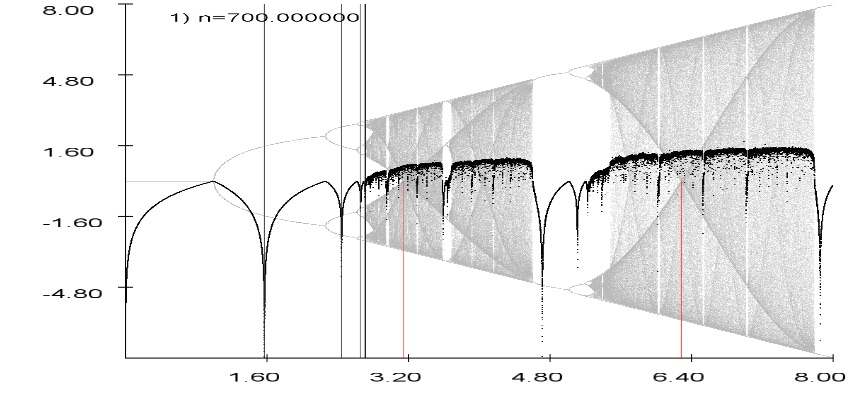
\includegraphics[scale=0.55]{bifurkation-sin}
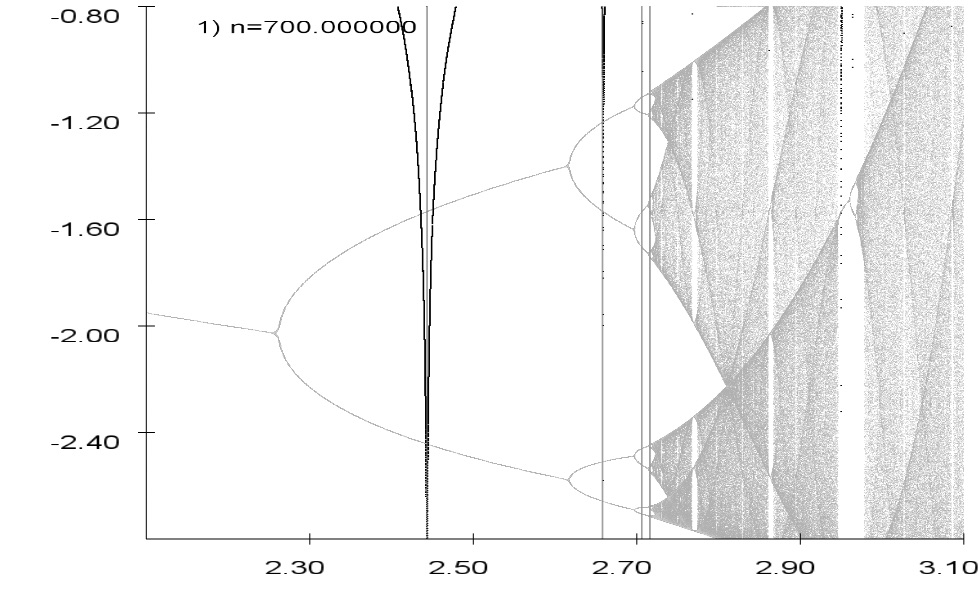
\includegraphics[scale=0.47]{bifurkation-sin-zoom}
\caption{Oben: Analyse des Bifurkationsdiagrammes der sinus Abbildung. Eingezeichnet sind die y=0 Achse, sowie die ersten 6 Superattraktiven Stellen für r (Erste Superattraktive Stelle bei $r=0$. Ebenfalls wurden $\pi$ und $2\pi$ eingezeichnet. Unten: Vergrößerung des Ausschnittes $r \in [2.1,3.1], y\in[-2.8,-0.8]$}. 
\label{fig:bifurc-sin}
\end{figure}

 
\section { Duffing-Gleichung}
Wir betrachten nun einen angetrieben und gedämpften Oszillator. Als Unterschied zum gewöhnlichen Harmonischen Oszillator tritt hier ein kubischer Dämpfungsterm auf.
$$\ddot{x}+\lambda\dot{x}+\beta x^3=\epsilon\cos{\Omega t}$$
Diese DGL lässt sich nun nicht mehr analytisch berechnen.
Im Folgenden lösen wir die Gleichung mit der Euler-Methode (REFERENZ: Euler...) als auch mit dem Runge-Kutta Verfahren (REFERENZ: Runge...).
$$\frac{dy}{dt}=\epsilon\cos{\theta}-\lambda y - \beta x^3$$
$$\frac{dx}{dt}=y$$
$$\frac{d\theta}{dt}=\Omega$$
\subsection { Attraktoren }
Im folgenden verwenden wir als Parameter $\epsilon = 0,2$, $\lambda = 0,08$, $\beta = 1$ und $\Omega = 1$
Zunächst untersuchen wir die Unterschiede der verwendeten numerischen Verfahren bei gleich bleibenden Anfangswerten. Dazu wählen wir $x_0=0.21$ und $y_0=0.02$ und betrachten das Phasendiagramm bei unterschiedlichen Schrittgrößen $h$.


- Unterschiede Runge Kutta Euler (unterschiedliche attraktoren)
\newline
- stabile / instabile Trajektorien --> parameter $h = \frac{Zeit}{Iterationen}$
\newline
- Optimierung durch Schrittweiten adaptierung
\newline
- lyapunov??
\subsection{ Poincareschnitt }
Die gezeigten Phasenraumportaits sind Projektionen des dreidimensionalen Phasenraums $(x,y,\theta)$ auf die $(x,y)$ Ebene. Der Poincaree Schnitt ist eine Abbildung aller $(x,y)$ welche eine bestimmte Ebene im Phasenraum schneiden. In Abbildung XYZ ist ein Bereich Poincaree Schnitt des Duffing-Oszillators mit $\epsilon=7.72$ und $\theta=0$ gezeigt. Zur Implementation des Poincaree Schnittes wählten wir $\theta=0$ um die Praktikumsanleitung als Test unserer Software nutzen zu können. Dabei nutzten wir $sin(\theta_1)*sin(\theta_2) \leq 0.0 \iff Ebenenschnitt$:
\begin{lstlisting}
      pos = sin(theta);
      if (last_pos*pos <= 0.0f) {
          result[k*2] = last_x;
          result[k*2+1] = last_y;
          k++;
      }
      last_pos = pos;

\end{lstlisting}
Dieses Verfahren zeigt bei genauerer Betrachtung aber leichter Ungenauigkeiten. So wird nicht exakt das $(x,y)$ duplet abgebildet bei welchen die Ebene geschnitten wurden, stattdessen wird das $(x,y)$ Duplet bei $\theta_2$ angezeit. Eine Möglichkeit dies zu Optimieren wäre den Mittelwert $(\frac{x_1+x_2}{2}, \frac{y_1 + y_2}{2})$ als Schnittpunkt zu identifizieren.
\begin{figure}
	\centering
	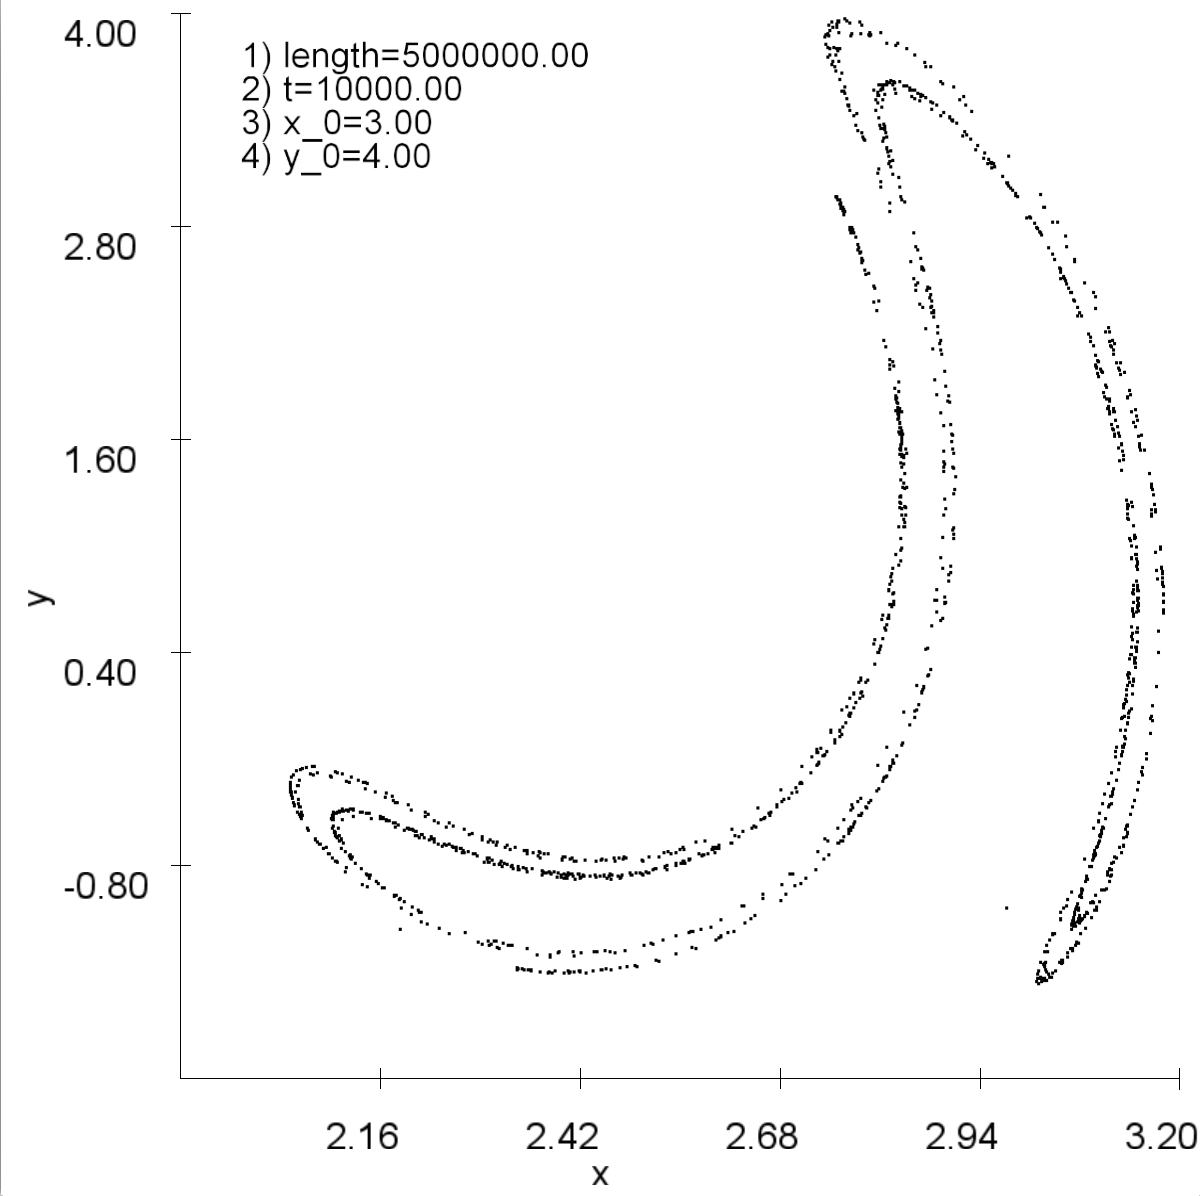
\includegraphics[scale=0.20]{poincare-772}
	\caption{Poincare Schnitt des Duffing Oszillators für $\epsilon=7.72 x=3.0, y=4.0, \lambda=0.2, \beta=1, \theta=1$. als Referenz aus dem VORBEREITUNGSHEFT-LITERATUR-S38}
	\label{img:poincare-772}
\end{figure}


\section {LDR-Oszillator}
Im folgenden untersuchen wir einen realen nichtlinearen Schwingkreis.

TODO: Schaltskizze
\subsection { Theorie } \label{ssec:theo}
Zunächst lässt sich ein linearer Schwingkreis der aus einem Widerstand, einem Kondensator und einer Spule besteht über die Spannungen an den einzelnen Bauteilen beschreiben
$$V_g=V_c+V_l+V_r \text{ (Kirschoff'sches Gesetz)}$$
Daraus folgt mit $V_g=V_s\cos{\omega t}$ die Differentialgleichung
$$\ddot{Q}L + \dot{Q}R+ \frac{Q}{C} = V_s\cos{\omega t}$$
welche mit dem angetriebener, gedämpfter Oszillator vergleichbar ist. Dabei ist $Q$ die Ladung, $L$ die Induktivität der Spule, $R$ der Widerstand, C die Kapazität des Kondensators $V_s$, die angelegte Spannung und $\omega$ die Frequenz der angelegten Wechselspannung.
\newline
Wird nun der Kondensator durch eine Diode ausgetauscht erhalten wir, wie bei Duffing-Oszillator, einen nichtlinearen Term. Während beim linearen Schwingkreis $I=\frac{dQ}{dt}$ gilt lässt sich die Diode als parallel geschalteter Kondensator und Widerstand mit 
$$I=I_f(1-\exp(-\frac{V_d}{V_t})) + \frac{dQ}{dt}$$
beschreiben, wobei $I_f$ und $V_t$ Konstanten sind.
Dies führt zu
$$\frac{dV_d}{dt}= \frac{I-I_f(1-\exp(-\frac{V_d}{V_t}))}{C_f\exp(-\frac{V_d}{V_t})} $$
in Durchlassrichtung und 
$$\frac{dV_d}{dt}= \frac{I-I_f(1-\exp(-\frac{V_d}{V_t}))}{C_r(1+\frac{V_d}{\phi})^{\gamma}}$$
in Sperrrichtung.
Weiterhin gilt
$$\frac{dI}{dt}=\frac{V_s \cos{\theta} - V_d - RI}{L}$$
$$\frac{d\theta}{dt}=\omega$$
Damit lässt sich nun das Euler-Verfahren anwenden (siehe \ref{ssec:num})

\subsection{ Numerische Berechnungen } \label{ssec:num}
Unter Verwendung folgender Paramter
\begin{center}
    \begin{tabular}{ | l | l | p{5cm} |}
    \hline
    $R$ & $100\Omega$ & beschreibung \\ \hline
    $L$ & $2367\cdot10^{-6} H$ & beschreibung \\ \hline
    $C_r$ & $82 pF$ & beschreibung \\ \hline
    $C_f$ & $56 \cdot10^{-6}  pF$ & beschreibung \\ \hline
    $I_f$ & $2,8pA$ & beschreibung \\ \hline
    $\gamma$ & $0,44$ & beschreibung \\ \hline
    $\phi$ & $0,6V$ & beschreibung \\ \hline
    $V_t$ & $34mV$ & beschreibung \\
    \hline
    \end{tabular}
\end{center}

haben wir für unterschiedliche Anregungsspannungen $V_s$ numerisch die Gleichungen aus  \ref{ssec:theo} gelöst. Dabei sind wir davon ausgegangen, dass für $V_d > -0.6$ die Diode sperrt und ansonsten leitet.
\newline
Für unterschiedlichen Anregungsspannungen erhalten wir teilweise deutliche Akttraktoren als auch chaos (siehe Abbildung \ref{fig:ldr-prd}).
\newline
\begin{figure}
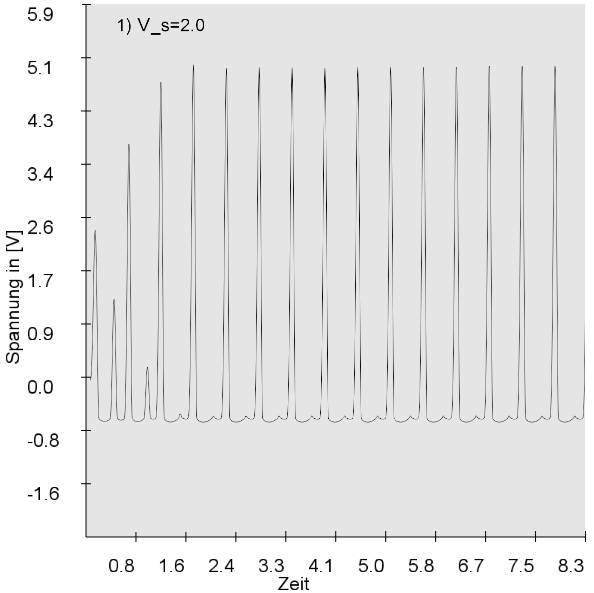
\includegraphics[scale=0.28]{V_s-2V_spannung}
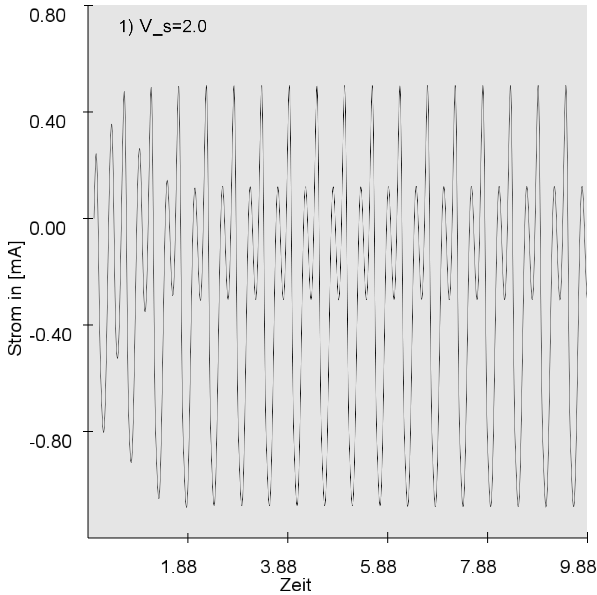
\includegraphics[scale=0.28]{V_s-2V_strom}
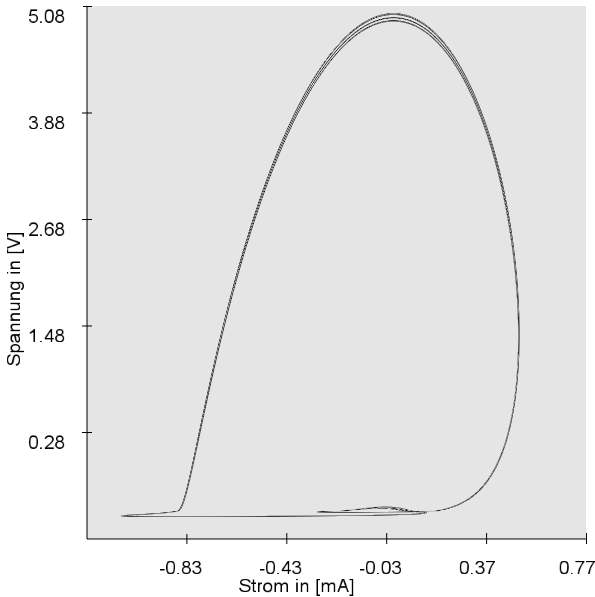
\includegraphics[scale=0.28]{V_s-2V}
\caption{LDR-Schwingkreis bei einer Anregungsspannung von $V_s=2V$. Numerisch mit Euler-Cauchy-Verfahren gelöst, bei einer Schrittweite $h=10^{-9}$ Links: Zeitlicher Verlauf der Spannung $V_d$ an der Diode ($10^5$Iterationen). Mitte: Zeitlicher Verlauf des Stroms $I$ ($10^5 Iterationen$). Rechts: Phasenraumdiagram nach $10^5$ Iterationen für weitere $4 \cdot 10^5$ Iterationen }. 
\label{fig:ldr_v2}
\end{figure}

\begin{figure}
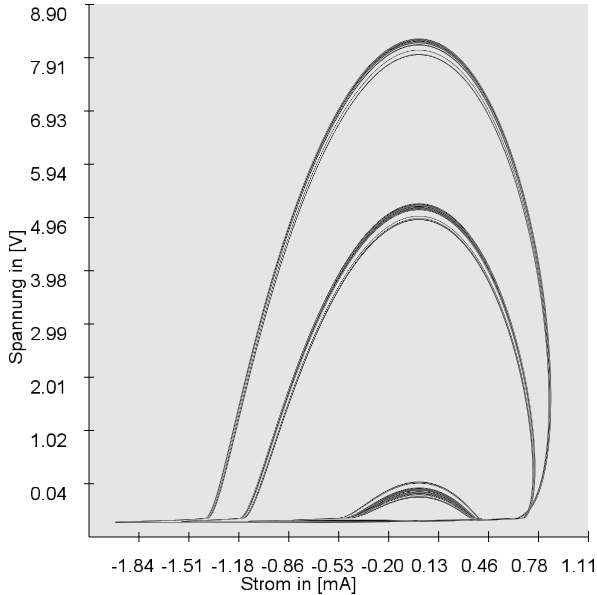
\includegraphics[scale=0.28]{V_s-4V}
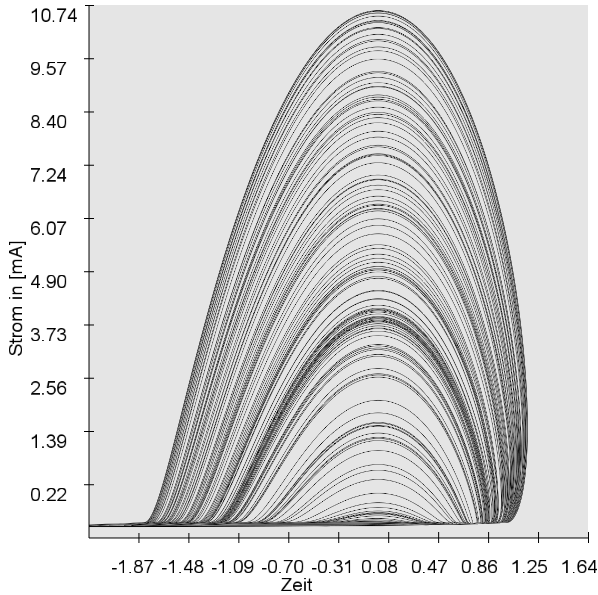
\includegraphics[scale=0.28]{V_s-6V}
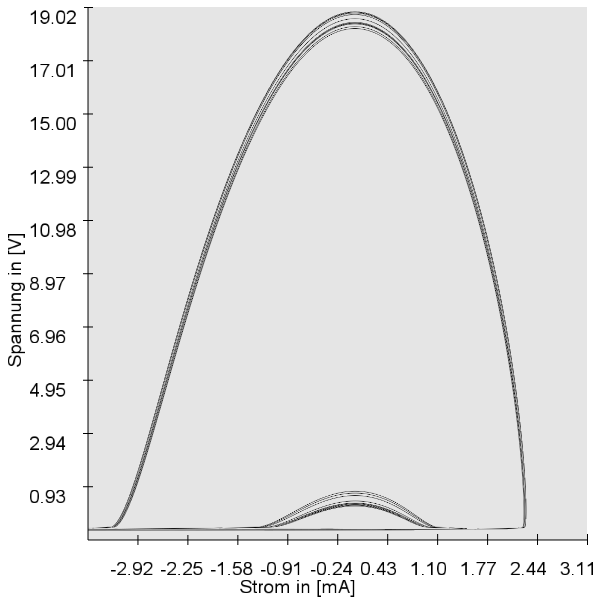
\includegraphics[scale=0.28]{V_s-15-67V}
\caption{Phasenraumdiagramme bei unterschiedlichen Anregungsspannungen $V_s$ nach $10^5$ Iterationen für weitere $4 \cdot 10^5$ Iterationen. Links: $V_s=4V$. Mitte: $V_s=6V$. Rechts: $V_s=15.67V$}
\label{fig:ldr-prd}
\end{figure}

\begin{figure}
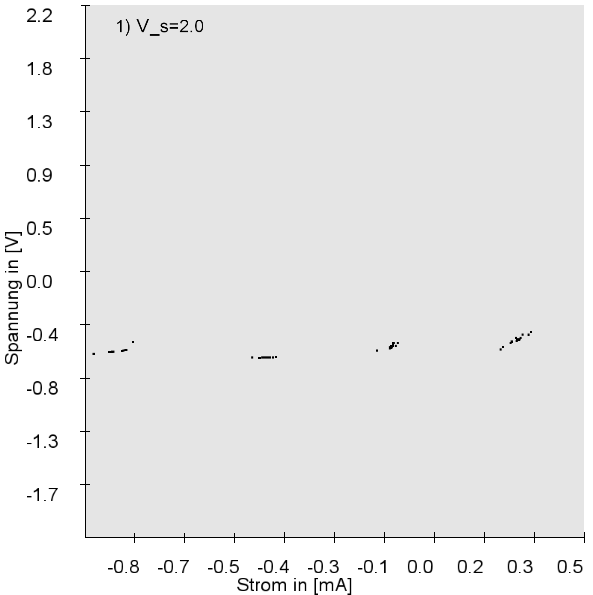
\includegraphics[scale=0.5]{Poincare-nach10000iterations}
\caption{Poincaré-Schnitt für $V_s=2V$ durch die Ebene bei $\sin(\theta)=0$ angefangen nach $10^4$ Iterationen. Insgesamt 1500 Punkte}
\label{fig:ldr-prd}
\end{figure}


\subsection{ Versuchsaufbau}
Der in diesem Versuch verwendete Schwingreis ist aufgebaut aus einer Spule, einem Widerstand und einer Diode.....

\subsection { Versuchsdurchführung }

\subsection { Zusammenfassung }

\section{ Literatur }
\begin{itemize} 
\item Nichtlineare Dynamik und Chaos - Physikalisches Praktikum für Fortgeschrittene Universität Hamburg
\end{itemize}




\end{document}







